\chapter{Diffusion measurements at the CERN LHC}\label{ch:diffusion_meas}
\noindent\textsf{The content of this chapter, with the due adaptations, has resulted in the proceedings by C.\ E.\ Montanari, A.\ Bazzani, M.\ Giovannozzi, A.\ A.\ Gorzawski, and S.\ Redaelli \textit{\citetitle{montanari:ipac22-mopost043}}, which were presented as a poster at IPAC'22 in June 2022~(Ref.~\cite{montanari:ipac22-mopost043}).}

\vspace{3em}

In Chapter~\ref{ch:probing}, we presented an optimal method to measure the diffusion coefficient of a beam halo, based on the characteristics of the outgoing current, given by a Fokker-Planck equation with a Nekhoroshev-like diffusion coefficient. In this chapter, we apply this method to the available LHC collimator scan data, which was gathered during Run~2, however, not using the optimised measurement protocol devised in the previous chapter.

As this measurement campaign was tailored to a different model of diffusion, the data was gathered with a different protocol, which inevitably does not meet all the optimal requirements highlighted in the previous chapter. This inevitably required an adjustment of the reconstruction procedure to account for the differences between the optimal and the actual measurement protocol.

The chapter is structured as follows. In Section~\ref{sec:4:collimation}, we present the LHC collimation system. In Section~\ref{sec:4:analysis}, we present the collimator scan data and the diffusion coefficient reconstruction, together with the necessary adjustments applied to the reconstruction procedure to account for the differences between the optimal and the actual measurement protocol. Finally, some conclusive remarks are given in Section~\ref{sec:4:remarks}.

\section{The LHC collimation system}\label{sec:4:collimation}

The LHC layout~\cite{Bruning:782076} can be summarised in a geometric scheme composed of eight straight insert regions (IR) and eight circular arc segments. A simple scheme of this layout is reported in Fig.~\ref{fig:lhc_layout}, left. Within this circular scheme, the main particle physics experiments are located in IR1, IR2, IR5 and IR8, namely, ATLAS~\cite{TheATLASCollaboration_2008}, ALICE~\cite{Alessandro:879894}, CMS~\cite{Chatrchyan:1129810}, and LHCb~\cite{Alves:1129809}. In these four IRs, the two beams intersect and interact in what is referred to as an Interaction Point (IP). The RF cavities for accelerating the beams are in IR4 and IR6 hosts the beam extraction system. Finally, IR3 and IR7 are dedicated, respectively, to the longitudinal and transverse collimation system.

\begin{figure}[hpt]
    \centering
    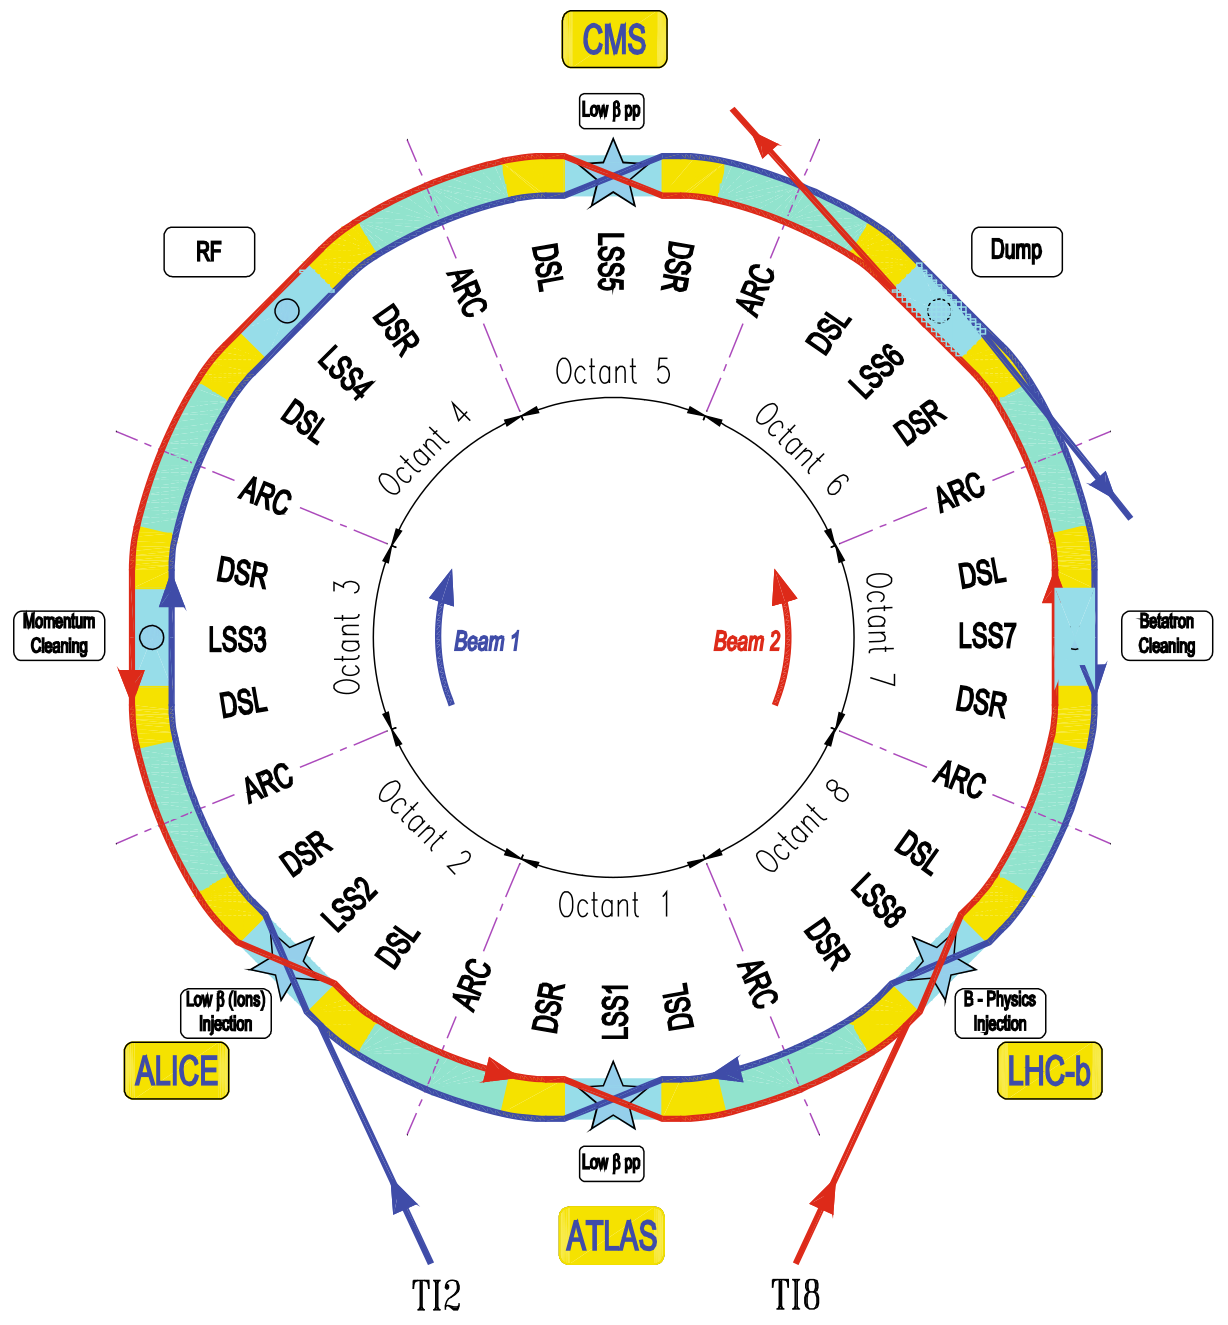
\includegraphics[width=0.49\textwidth]{5_Diffusion_measurement_LHC/figs/layout.png}
    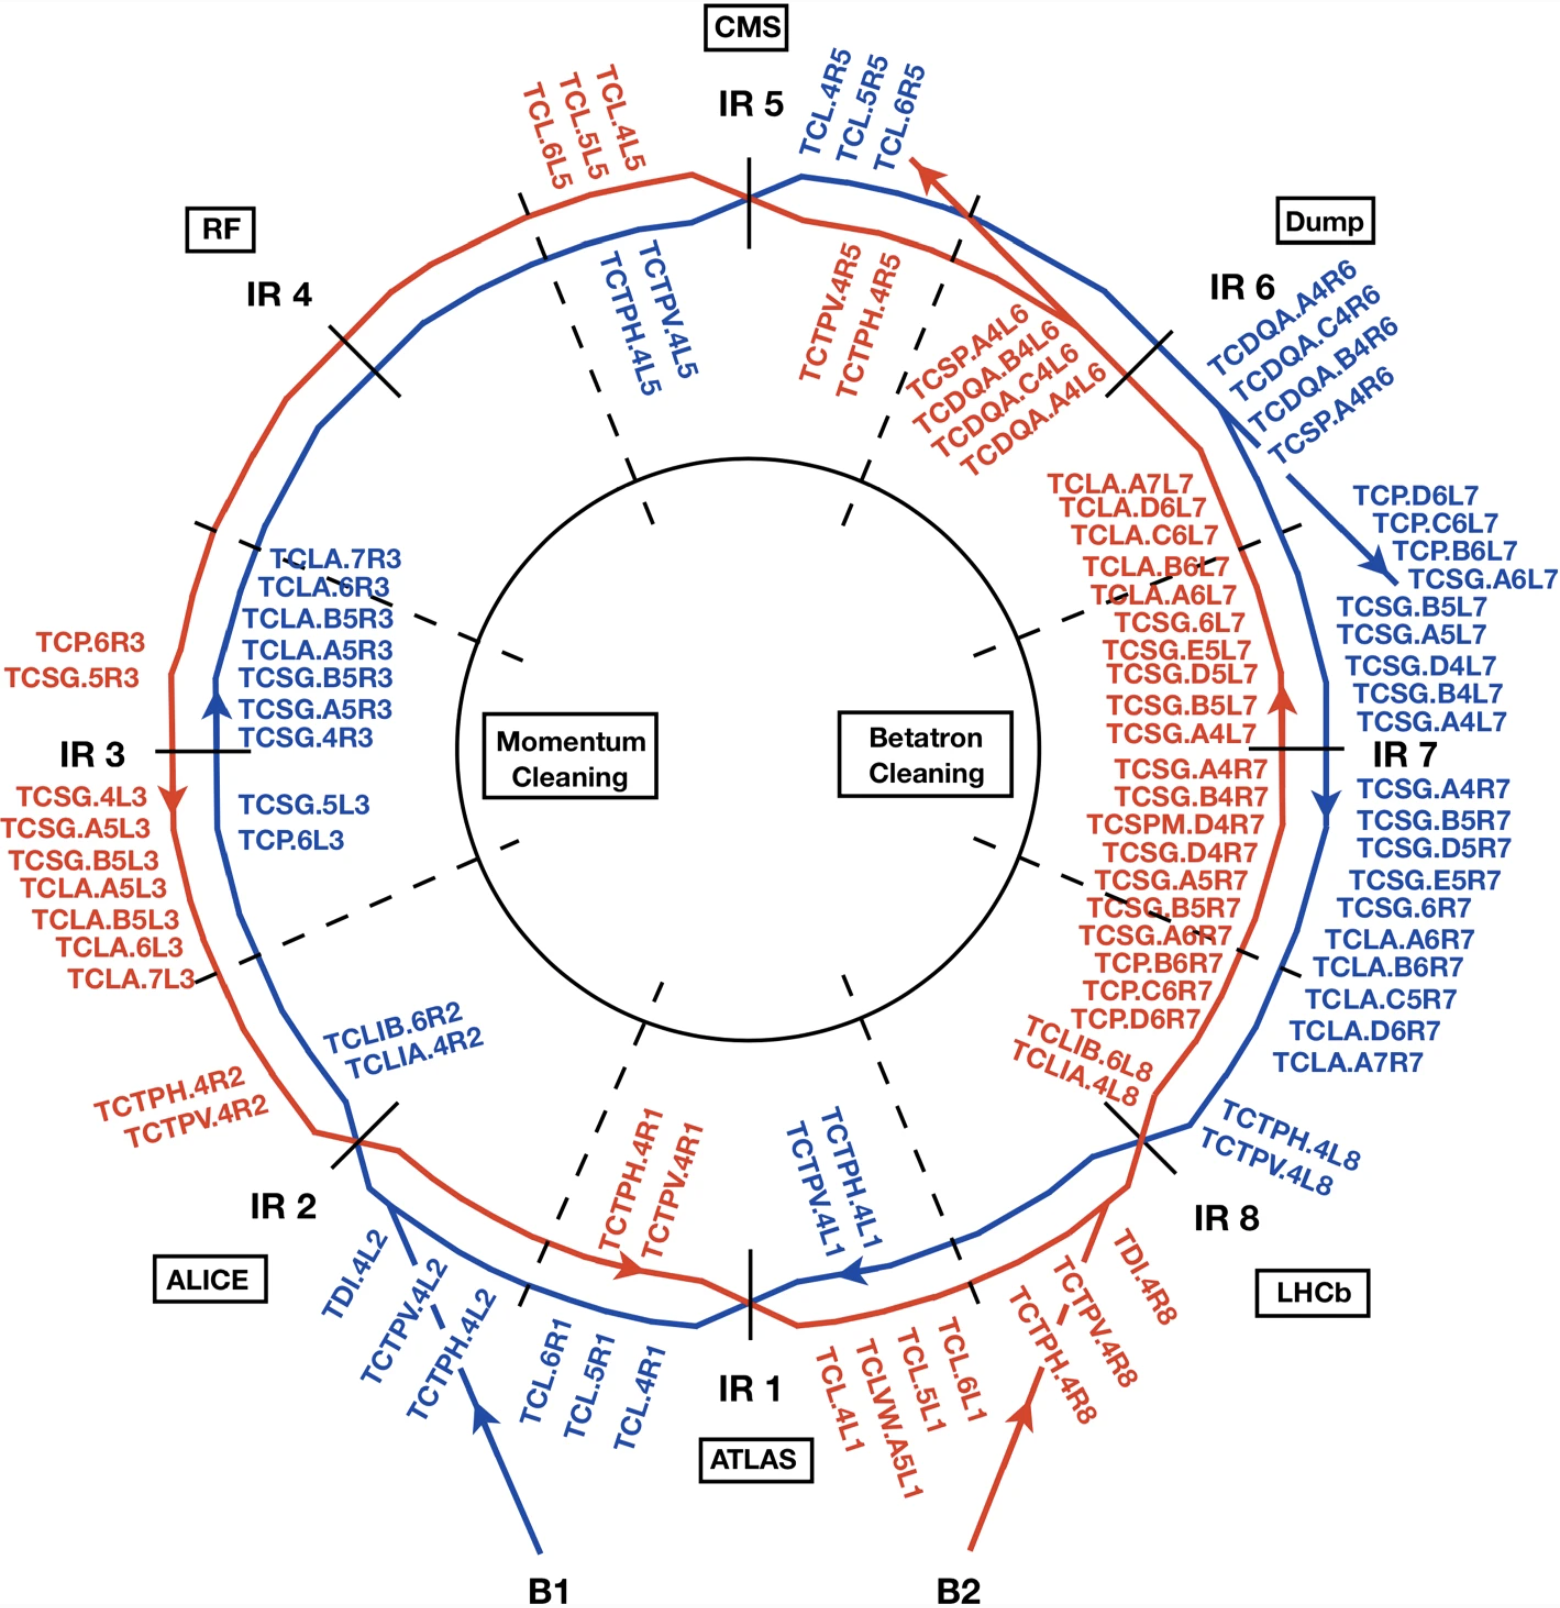
\includegraphics[width=0.49\textwidth]{5_Diffusion_measurement_LHC/figs/coll_scheme.png}
    \caption{Left, layout of the LHC. The ring follows an eightfold symmetry. Each octant hosts a Long Straight Sector (LSS) surrounded by two Dispersion Suppressor regions (DSR and DSL). Each octant is connected by an arc (ARC). (From Ref.~\cite{Bruning:782076}). Right, LHC collimation system layout in blue and red for Beam~1 and Beam~2, respectively. (From Ref.~\cite{azzopardi:crosstalk})}
    \label{fig:lhc_layout}
\end{figure}

The LHC collimation system is a fundamental component of machine operation and safety~\cite{1590664, Assmann:972336}. It has multiple functions, such as cleaning the beam halo, protecting the machine against unexpected and anomalous losses~\cite{BRUCE201719}, and reducing the background noise in experimental IPs~\cite{Bruce:1646958, Bruce:2686581}.

The collimation system counts more than 120 individual collimators. Most of these collimators are movable devices made up of two movable jaws made of solid material, which can be brought at different distances from the circulating beam~\cite{Bertarelli:794628}. A summary of the various collimators positioned along the LHC layout is reported in Fig.~\ref{fig:lhc_layout}, right. These jaws are straight and parallel to the beam and have a tapering at both ends, along the axis of the beam. The distance between the start and end of the tapering, where the jaw material is straight, is called the active length of the collimator. Some photos and schemes of these LHC collimators are reported in Fig.~\ref{fig:collimator_pics}.

\begin{figure}[hpt]
    \centering
    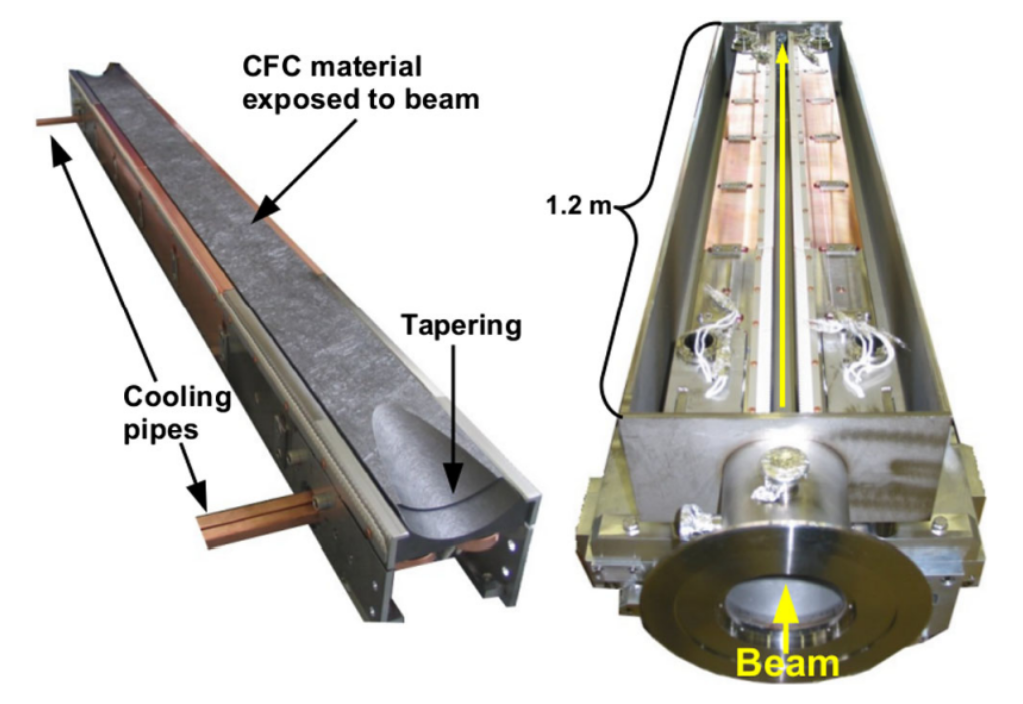
\includegraphics[width=0.75\textwidth]{5_Diffusion_measurement_LHC/figs/collimator_pics.png}
    \caption{Left picture, jaw of a secondary collimator, made of carbon-fiber composite (CFC) and water cooled through copper pipes. Right picture, two collimator jaws are installed in a collimator tank. (From Ref.~\cite{bruce2014simulations})}
    \label{fig:collimator_pics}
\end{figure}

At IR7, where the betatronic collimation system is located, we have an effective cleaning stage of halo particles that happen to have an excessively large amplitude of the betatron oscillation. This is called \textit{betatron cleaning}. To achieve effective betatron cleaning, we require that the magnetic lattice optics in the collimation region has very low dispersion and high $\beta$ function values. With such an optics setup, particles with high transverse displacement also feature high betatron displacement.

In IR3, instead, a \textit{momentum cleaning} of particles takes place. In that region, conversely, a high dispersion value is kept, so that the high transverse displacement is mainly caused by high momentum offset.

To safely clean the beam halo without damaging the magnets or other components of the machine, the LHC collimation system works on the basis of a multistage process. This multistage process consists of a \textit{hierarchy} of individual collimators with the purpose of progressively cleaning and controlling the loss of particles. A scheme of this hierarchy is presented in Fig.~\ref{fig:collimator_hierarchy}.

\begin{figure}[hpt]
    \centering
    \def\svgwidth{1.0\columnwidth}
    \import{5_Diffusion_measurement_LHC/figs}{hierarchy.pdf_tex}
    \caption{Scheme of the multistage collimation system in the LHC. The hierarchy includes primary (TCP), secondary (TCSG) and tertiary (TCT) collimators and shower absorbers (TCLA). Particles in the primary halo interact with the TCP and are scattered to the TCSGs. The hadronic showers coming from the TCSGs are finally absorbed by the TCLAs, and TCTs are in place to protect the aperture bottlenecks of the triplet quadrupoles. Part of the secondary halo interacts with the ionization chambers of the BLMs, and provide an indirect measurement of the primary halo. (Scheme based on Ref.~\cite{Hermes:2241364})}
    \label{fig:collimator_hierarchy}
\end{figure}

Primary collimators, which are also known as \textit{Target Collimator Primary} (TCP), are those placed closest to the edge of the beam and form the first stage of collimation. The purpose of this first collimation stage is to intercept and dispose of beam halo particles, i.e.\ it is the stage at which the beam halo actually gets intercepted above a certain threshold. When interacting with the primary collimator matter, the primary particles may exhibit various scattering behaviours, from acquiring an angular kick to depositing energy and producing secondary particles. 

These particles, scattered by the TCPs, form the secondary halo, which is then tackled by the secondary collimators \textit{Target Collimator Secondary-Graphite} (TCSG). The particles leaving the collimator finally form the tertiary halo, which finally interacts with the active absorbers, \textit{Target Collimator Long Absorber} (TCLA), which are installed downstream of the TCSGs, and \textit{Target Collimator Tertiarys} (TCTs), which make up a third final collimation stage for local protection for the aperture bottlenecks in the machine, i.e.\ in the triuplet quadrupoles.

Such a hierarchy offers various advantages over a simple single-stage collimation system. It ensures that particles that have been incorrectly outscattered at larger amplitudes and modified energies, constituting the so-called \textit{secondary beam-halo}, will be mainly absorbed by the next stages of collimation and not by other fragile parts of the machine. Moreover, the interaction of beam-halo particles with the primary collimator produces hadronic showers whose products can reach the cold magnets downstream of the cleaning region, possibly leading to unwanted quenches.

In IR7, there are 3 sets of collimators that cover the horizontal, vertical, and skew planes, as they have been shown to provide satisfactory cleaning~\cite{Jeanneret:368725}. The collimator hierarchies for these planes are, respectively, denominated by the letters C, D, and B. That is, the horizontal target primary collimator is called TCP.C. In IR3, the dispersion is only in the horizontal plane and only one set of collimators is installed to perform the longitudinal cleaning.

A multi-stage collimation system allows one to distribute the beam loads over a large controlled area. However, it also leads to a significant increase in the machine impedance, i.e.\ the level of self-interaction of the charged particle beam, mediated by the machine environment~\cite{Wiedemann2007}, which can be an important cause of beam instability and losses. Collimators are the single highest contributors of LHC impedance at top energy~\cite{Mounet:1451296}, as their resistive wall tends to be the element closest to the beam. Therefore, a multi-stage collimation system has to be configured so that it balances beam load distribution and impedance contributions efficiently. Active studies are ongoing to optimise the collimation system to minimise the beam losses and the machine impedance, see, e.g.\ Ref.~\cite{Antipov:2648423}.

The secondary particle showers represent the point of observation to measure the amount of primary particles absorbed by the TCPs. To quantify this amount, the LHC is equipped with multiple ionisation chambers, which make up the beam loss monitor (BLM) system~\cite{blmSystem1, blmSystem2}. The charged particles that pass through the ionisation chambers finally provide a measure of \SI{}{Gy \per s}, which can be converted into a corresponding measure of \SI{}{protons \per s} lost using a measured calibration factor, evaluated by controlled collimator-induced losses~\cite{arek}, which are also quantified in parallel by the \textit{DC Beam Current Transformer} (DCBCT)~\cite{Denard:1213275}, which measures the number of protons in the circulating beam by measuring the magnetic field, induced by the moving beam. A picture of an LHC BLM is presented in Fig.~\ref{fig:blm}. The calibrated BLM data are the precise loss signal that we finally expect to use to reconstruct the diffusion behaviour in the transverse plane.

\begin{figure}[hpt]
    \centering
    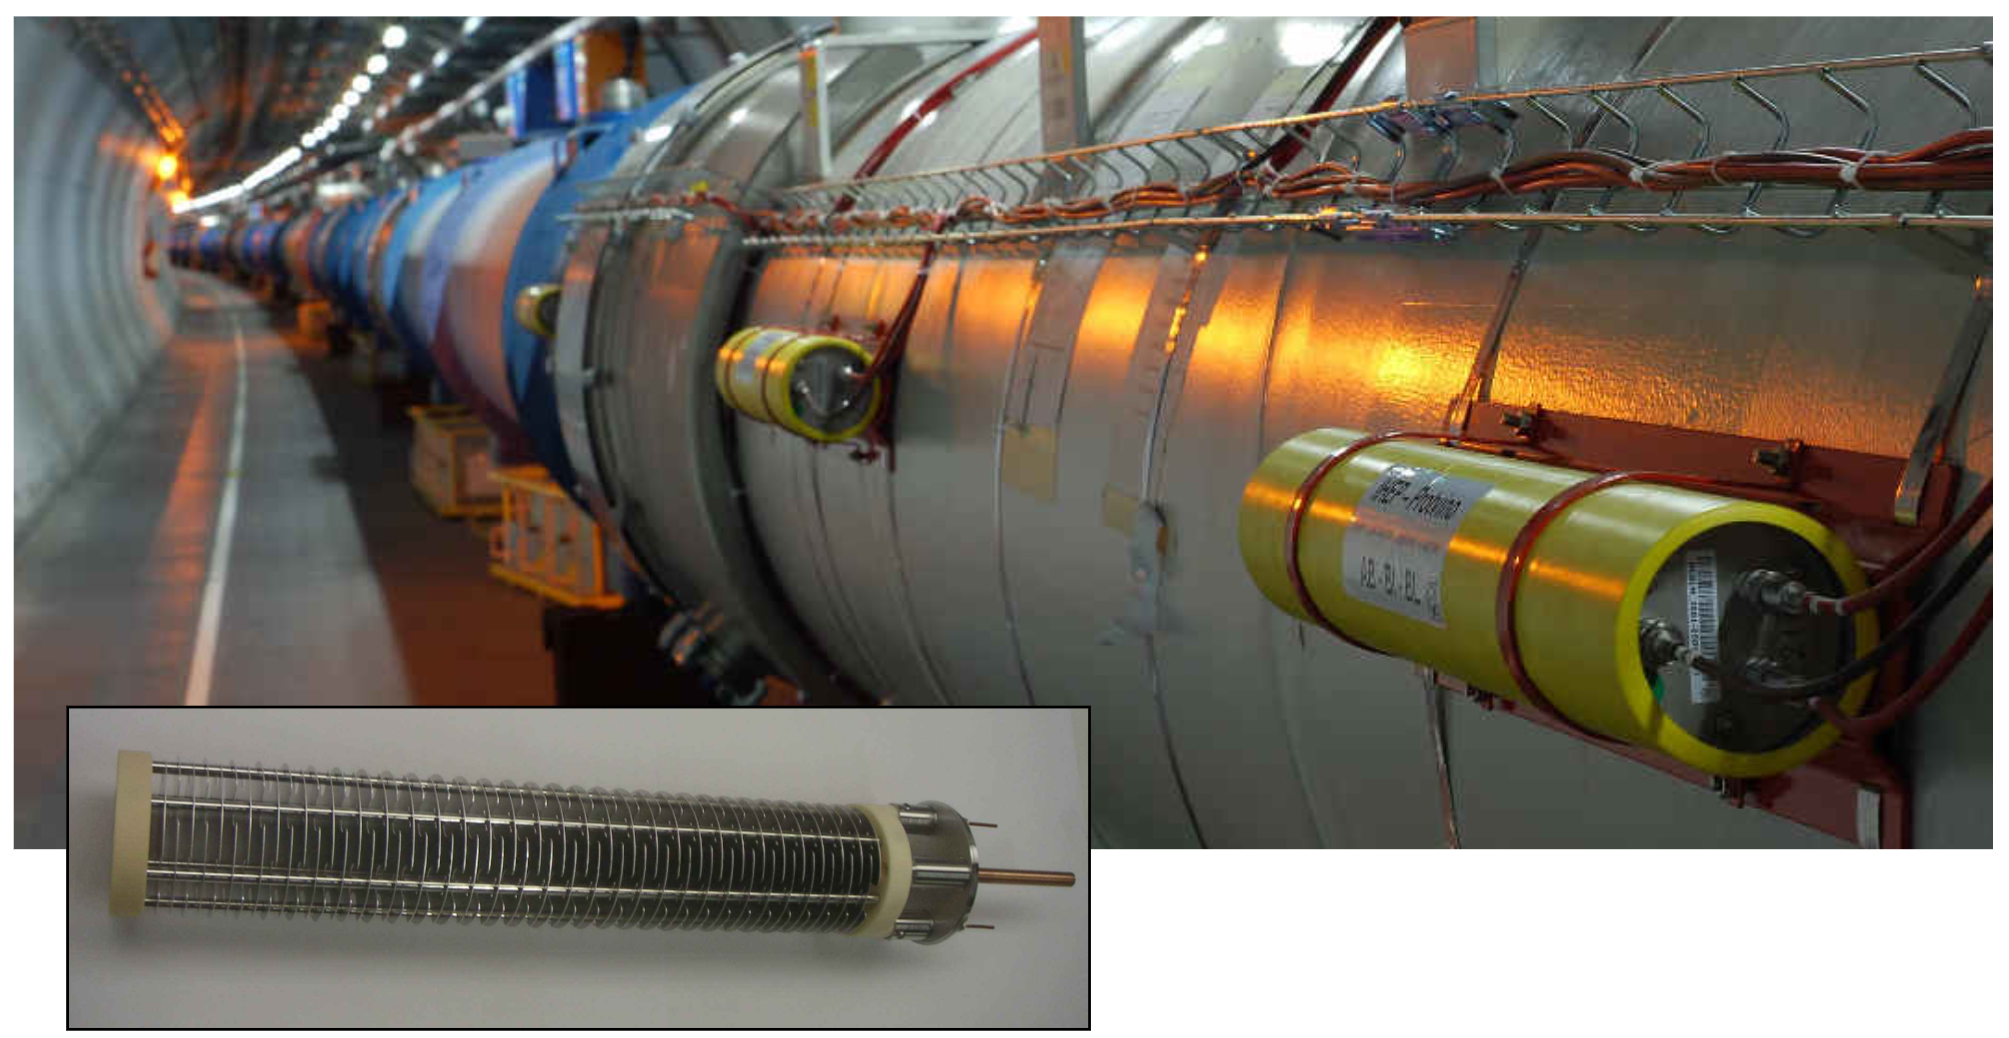
\includegraphics[width=0.75\textwidth]{5_Diffusion_measurement_LHC/figs/blm.png}
    \caption{Top picture, ionization chambers of the LHC BLM system, mounted on the side of the LHC Magnets. Bottom picture, inner structure of a BLM ionization chamber. (From Ref.~\cite{blmonline})}
    \label{fig:blm}
\end{figure}
%
\section{Analysis of experimental data}\label{sec:4:analysis}
%
Between 2016 and 2018, collimator scans were performed at the CERN LHC with physics beams at \SI{6.5}{TeV}~\cite{PhysRevAccelBeams.23.044802}. During these scans, one of the jaws of the primary collimators in IR7 was moved inward and outward in small steps, starting at $~5\sigma_\text{nom}$, where the nominal sigma value $\sigma_\text{nom}$ is evaluated for a nominal emittance $\varepsilon_\text{nom} =$ \SI{3.5}{\micro\meter}.

The scan was performed after executing a beam-based alignment~\cite{valentino2012semiautomatic} of the collimator, which is a procedure in which the TCP jaws are progressively positioned closer to the beam until the halo is touched. By performing such a procedure, one is sure that the centre of the collimator gap is precisely positioned around the local closed orbit.

The measurement is performed with the local beam loss monitoring (BLM) system and is provided in unit of \SI{}{Gy \per s} with \SI{1}{Hz} sampling rate, processed over different \textit{Running Sums} (RS), evaluated by a real-time processing system implemented on FPGA~\cite{4179157}. In this implementation, a time window is moved over the signal sampled by the device, and the maximum peak measured in the time window is considered the final measurement, which is finally reported in \SI{}{Gy \per s}, RSs range from a minimum of \SI{40}{\micro s} to a maximum of \SI{83.89}{s}. A list of the various RS defined in the measurement system is presented in Table~\ref{tab:rs_scheme}.

\begin{table}[hpt]
    \centering
    \scalebox{0.80}{
    \begin{tabular}{c|c|c|c|c|c|c}
    \toprule
        \multirow{2}{*}{\makecell{Signal\\Name}} & \multicolumn{2}{c|}{Time Windows} & \multicolumn{2}{c|}{Refreshing} & \multicolumn{2}{c}{Data formats} \\
        \cline{2-7}
        & \makecell{Number\\of \SI{40}{\micro s}\\steps} 
        & \makecell{Duration\\$[$\SI{}{ms}$]$} 
        & \makecell{Number\\of \SI{40}{\micro s}\\steps} 
        & \makecell{Duration\\$[$\SI{}{ms}$]$} 
        & FPGA/VME 
        & \makecell{Measurement\\and Logging DB\\(rate: \SI{1}{Hz})\\$[$\SI{}{Gy \per s}$]$}\\
        \midrule
        RS01 & $1$ & $0.04$ & $1$ & $0.04$ & \multirow{8}{*}{\makecell{Maximum of\\sum values\\observed\\from the\\last\\readout}} & \multirow{8}{*}{\makecell{Maximum of\\sums\\normalized\\to window\\length}} \\
        RS02 & $1$ & $0.08$ & $1$ & $0.04$ & & \\
        RS03 & $2$ & $0.32$ & $1$ & $0.04$ & & \\
        RS04 & $8$ & $0.64$ & $1$ & $0.04$ & & \\
        RS05 & $16$ & $2.56$ & $2$ & $0.08$ & & \\
        RS06 & $64$ & $10.24$ & $2$ & $0.08$ & & \\
        RS07 & $256$ & $81.92$ & $64$ & $2.56$ & & \\
        RS08 & $16384$ & $655.36$ & $64$ & $2.56$ & & \\
        \midrule
        RS09 & $32768$ & $1310.72$ & $2048$ & $81.92$ & \multirow{4}{*}{\makecell{\footnotesize Last calculated\\ \footnotesize sums observed\\\footnotesize in the last\\\footnotesize readout}} & \multirow{4}{*}{\makecell{\footnotesize Last calculated\\\footnotesize sum normalized\\\footnotesize to window length}} \\
        RS10 & $131072$ & $5242.88$ & $2048$ & $81.92$ & & \\
        RS11 & $524288$ & $20971.52$ & $16384$ & $655.36$ & & \\
        RS12 & $2097152$ & $83886.08$ & $16384$ & $655.36$ & & \\
    \bottomrule
    \end{tabular}
    }
    \caption{Specifications of the various Running Sums (RSs) that are defined in the FPGA based data gathering system of the BLMs. (Ref.~\cite{rsdeftable})}
    \label{tab:rs_scheme}
\end{table}

\begin{figure}[hpt]
    \centering
    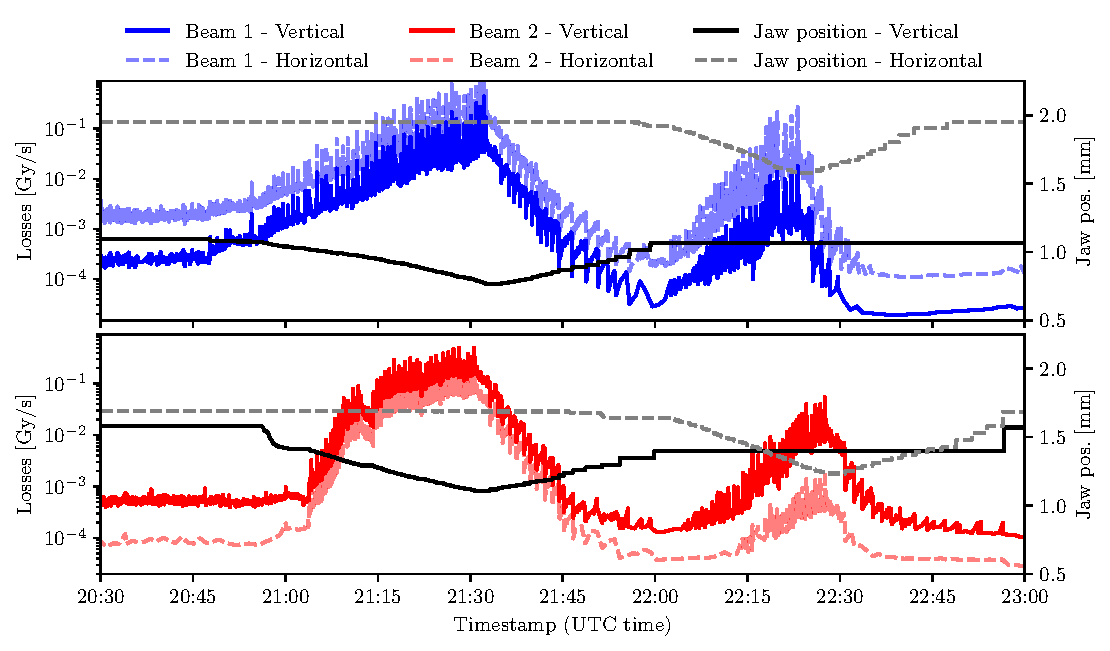
\includegraphics[width=\textwidth]{5_Diffusion_measurement_LHC/figs/raw.pdf}
    \caption{Beam loss data from the two separate BLM monitors corresponding to the TCPs on the vertical and horizontal planes, using RS06 (i.e.\ the maximum spike over a time window of \SI{10.24}{ms}), for Beam~1 and Beam~2, and positions of IR7 TCP jaws measured in the vertical and horizontal plane for the collimator scans carried out in fill 6052. The data acquired represent a complete collimator scan on both planes. The jaw positions are considered from the beam centre position, measured after a beam-based alignment. (Data from Ref.~\cite{PhysRevAccelBeams.23.044802})}
    \label{fig:raw_data}
\end{figure}

The IR7 TCPs dedicated to the vertical plane and to the horizontal plane (namely, TCP.D and TCP.C) were used to perform a collimator scan of the beam halo on both Beam~1 and Beam~2, performing a sequence of inward steps, with pauses of a few seconds between each step, followed by a train of outward steps, with pauses ranging from $\sim30$ seconds to almost two minutes between steps. The scraping was first performed on the vertical plane and then on the horizontal plane. 

During the scraping, the BLM data were recorded by the ionisation chambers placed after the collimator hierarchy. Two dedicated sets of BLMs are placed for the two separate planes and are considered in our analysis depending on the plane that is undergoing scraping. In Fig.~\ref{fig:raw_data} we present the data collected during fill 6052 of type RS06, i.e.\ sampling the maximum spike measured by the BLM over a time window of \SI{10.24}{ms}. Here, the collimator jaw positions are reported in millimetres from the centre of the beam, measured after the beam-based alignment. The two different BLM planes reading is reported.

It should be noted that these collimator scans were not performed using an optimal protocol such as that proposed in the previous chapter. In fact, complete inward scans, followed by outward scans, were used instead of a sequence of in/out steps. Furthermore, jaw movements were not always performed leaving enough time for the system to relax to its equilibrium state. This can be observed from the fact that, between most outward steps, the loss signal still has a non-negligible positive first derivative when the next collimator outward step is performed, suggesting that a recovery current process was still ongoing when the jaw was moved, as the expected global current process has negative or close to zero first derivative. This suggests that an ideal resting time between steps was not archived before the next collimator step.

Due to these two characteristics of the measurement protocol used during the collimation scan, some of the working hypothesis made in the previous chapter, which ultimately allow the reconstruction of $D(I)$ by fitting the normalised recovery current, may not hold. More specifically, we lack the upper bound to reconstruct the global current, and we cannot be sure that the beam tail distribution after an outward step follows Eq.~\eqref{eq:outward_difference}.

To address these characteristics and shortcomings of the data, we had to consider only a subset of the data and modify some of the elements of the fitting procedure. 

To address the lack of alternating jaw movements, we selected a region of interest (ROI) in which many outward steps were performed with almost regular sampling, with loss signals exhibiting the features we expect to see from a recovery current. This decision is motivated by the fact that the simulation study presented in the previous chapter shows how recovery currents induced by outward steps are much more reliable for reconstruction purposes than those induced by inward steps. 

In Fig.~\ref{fig:first} we present the portion of the data collected in Fill 6052 that we finally selected. Unfortunately, only the scraping performed in the vertical plane meets our quality requirements to apply the fitting of our diffusive model.

\begin{figure}[hpt]
    \centering
    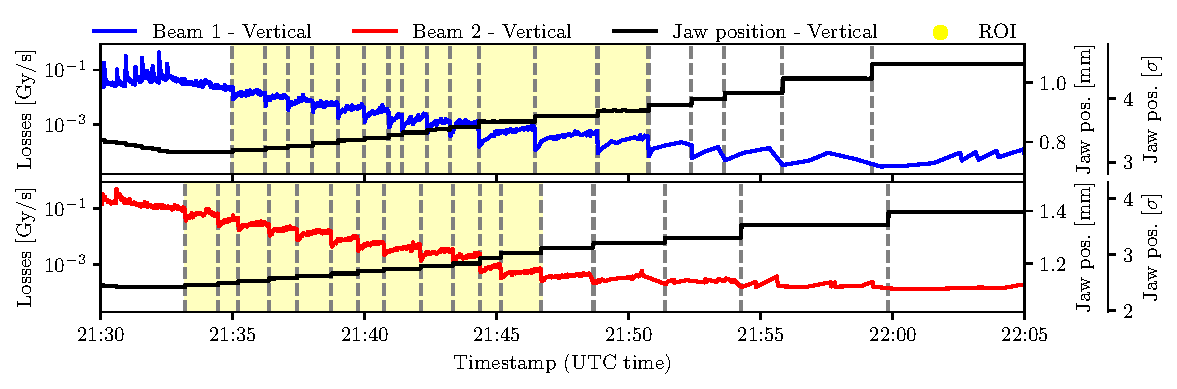
\includegraphics[width=\textwidth]{5_Diffusion_measurement_LHC/figs/first.pdf}
    \caption{Selected data from Fill 6052 (i.e.\ Fig.~\ref{fig:raw_data}). The data shown correspond to outward jaw movements in the vertical plane. The yellow-marked region of interest (ROI) represents a subset of data meeting our quality requirements for applying the fitting of our diffusive model. The jaw positions are considered from the beam centre position, measured after a beam-based alignment. A corresponding position measured in $\sigma$ units is also reported. (Data from Ref.~\cite{PhysRevAccelBeams.23.044802})}
    \label{fig:first}
\end{figure}

The measured collimator jaw position is converted to measured beam sigma units $\sigma$ using the nominal optical parameters and the measured value of the beam emittance, taking into account the position of the beam centre. The nominal optical parameters were considered as the measured $\beta$-beating level, i.e.\ the difference between the measured optical functions and the expected nominal values, was in the few percent level as expected from regular LHC operation~\cite{PhysRevAccelBeams.20.054801}.  To convert the \SI{}{Gy \per s} units of the BLM signal to \SI{}{protons \per s}, we used a calibration factor $F$~\cite{arek} dependent on the TCP jaw position. This calibration factor $F$ is calculated from the BLM loss data and the intensity lost recorded by the DCBCTs during the collimator steps. The coefficient reads 
\begin{equation}
    F = \left(-9.0\times10^{-14}\sigma + 6.2\times10^{-13}\right)^{-1} \,,
\end{equation}
where $\sigma$ is the position of the collimator jaw in sigma units.

The absence of alternating jaw movements implies a lack of information for constructing an upper-bound estimate of the global current. Moreover, since the jaw movements were not always performed to allow enough time for the system to relax to its semi-stationary state, we cannot make strong assumptions on the global current value by only interpolating the end points of the outward recovery currents. 

To address this issue, we define an initial estimate of the global current shape $J_\text{eq}^{\text{est}}(t)$, by constructing a Cubic Spline Interpolation (CSI) passing through the end points of the sequence of outward recovery currents, following the same methodology as presented in the previous chapter. This ``fundamental CSI'', has the features we expect to observe from a global current we expect to observe from a Nekhoroshev-like Fokker-Planck process. However, by just interpolating the end points, it does not take into account missing recovery due to collimator steps being performed too quickly.

To include this missing information, the fundamental CSI has been multiplied by different constant terms to represent possible different levels of partial recovery of $J_\mathrm{R}(t)$. This procedure is shown in Fig.~\ref{fig:second}. One can see how the fundamental CSI represents the initial lowest estimate of global current, while the different multiplicative constants introduce different gap levels after the terminating points of the recovery currents. This multiplicative can then be treated as a free parameter for reconstructing missing information.

%
\begin{figure}[hpt]
    \centering
    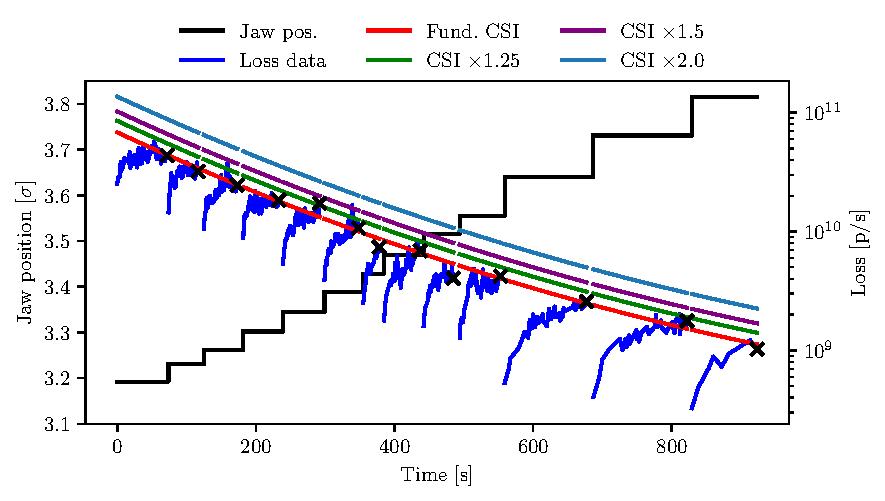
\includegraphics[trim={0 2.5mm 0 3mm}, clip, width=\columnwidth]{5_Diffusion_measurement_LHC/figs/second_bis.pdf}
    \caption{Possible estimates of $J_\mathrm{eq}(t)$ for Beam~1 data. An initial estimate is made starting from a Cubic Spline Interpolation (CSI) with positive second derivative passing through the end points of the measured recovery currents (red line). The various curves are obtained by multiplying the fundamental CSI by a constant term, and represent estimates of the partial recovery currents. The multiplicative constant considered is reported in the plot legend.}
    \label{fig:second}
\end{figure}
%

Finally, the rapid sequence of jaw movements introduces another issue: the difference distribution $\rho^\ast$ cannot be described with certainty by Eq.~\eqref{eq:outward_difference}, or its approximated form by Eq.~\eqref{eq:outward_difference_approx}. To address this issue, we replace the $D(I)$-dependent integral terms in Eq.~\eqref{eq:outward_difference_approx} with the approximation
\begin{equation}
    \rho_{\mathrm{app}}^{\ast}(I)= \begin{cases} -M & \text { if } I\leq I_{\mathrm{a}}\\ -\left(\frac{I_{\mathrm{a}}^{\prime }-I}{I_{\mathrm{a}}^{ \prime}-I_{\mathrm{a}}}\right) M & \text { if } I>I_{\mathrm{a}}  \end{cases} \, ,
    \label{eq:approximated_distribution_beam}
\end{equation}
where $M$ is a fixed constant for each jaw movement that represents an unknown amount of out-of-equilibrium distribution.

A scan is performed on different combinations of the multiplicative factor of the CSI and of $M$, while keeping track of the $\chi^2$ achieved by the fitting routine that determines the values of the model parameters $\kappa, I_\ast$. The result of this procedure is shown in Figs.~\ref{fig:fourth} and~\ref{fig:fifth}, where one can observe the existence of an optimal configuration of parameters and the good reconstruction performance achieved by such a configuration. The optimal fit results for Beam~1 and Beam~2 data are reported in Table~\ref{tab:fit_results}.

\begin{figure}[hpt]
    \centering
    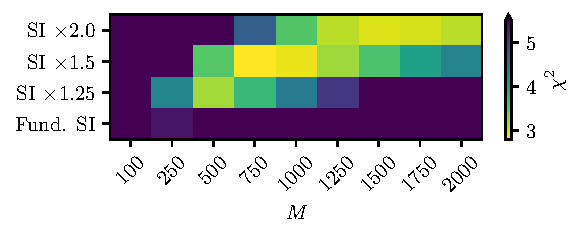
\includegraphics[trim={0 2.5mm 0 1.5mm}, clip, width=0.98\columnwidth]{5_Diffusion_measurement_LHC/figs/fourth.pdf}
    \caption{Fit performance of $\kappa$ and $I_\ast$ for Beam~1 data, using different combinations of CSI multiplicative constants and values of $M$ for Eq.~\eqref{eq:approximated_distribution_beam}. The color map shows the existence of an optimal pair of values at (CSI $\times 1.5$, $750$).}
    \label{fig:fourth}
\end{figure}
%
\begin{table}[hpt]
    \centering
    \begin{tabular}{lcccc}
        \toprule
        Beam / Plane & CSI & $M$ & $\kappa$ & $I_\ast\ [\sigma]$ \\
        \midrule
        Beam~1 / V & $\times1.5$ & $750$ & $0.59\pm0.03$ & $21\pm2$ \\
        Beam~2 / V & $\times1.5$ & $1000$ & $0.85\pm0.02$ & $39\pm8$ \\
        \bottomrule
    \end{tabular}
    \caption{Results of the fit procedure of $\kappa$ and $I_\ast$ for the selected data in the vertical plane, along with corresponding setup obtained for the CSI multiplicative constant and $M$ value for \eqref{eq:approximated_distribution_beam}.}
    \label{tab:fit_results}
\end{table}
%

Note that the values reported in~\cite{bazzani2020diffusion}, namely $\kappa=0.33 $ and $I_\ast \simeq 21$, were obtained for Beam~2 and considering the diffusion in the vertical plane. It should be stressed that these previous measurements were performed with non-colliding bunches, whereas in the beam measurements analysed here, beam-beam effects were present.

\begin{figure}[hpt]
    \centering
    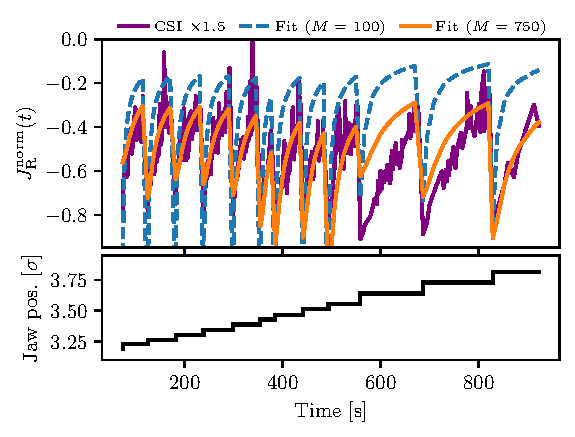
\includegraphics[trim={0 2.5mm 0 3mm}, clip, width=0.95\columnwidth]{5_Diffusion_measurement_LHC/figs/fifth.pdf}
    \caption{Fit results for Beam~1 data for two $M$ values, considering the recovery current obtained by using the optimal CSI multiplicative constant $\times 1.5$. The optimal $M$ value (orange) outperforms a lower $M$ value (blue) and manages to reconstruct the shape of the recovery currents.}
    \label{fig:fifth}
\end{figure}
%
\section{Final remarks}\label{sec:4:remarks}
%
Despite the differences between the approach used to collect the data during LHC Run~2 and the optimal one suggested by the numerical studies performed on the Nekhoroshev-like Forkker-Planck diffusive model, we were able to analyse the loss signal measured by the BLMs during collimator scans, and obtain a promising reconstruction of the recovery currents, which are ultimately the indicator of diffusive-like behaviour.

To address missing information in the data, due to the different measurement protocol used, we had to adapt some of the key elements of our fitting procedure. That is, we had to define a new method for reconstructing the global current estimate and we had to consider a different form for the difference distribution $\rho^\ast$. This led to good reconstruction performances and promising insights into the global diffusive behaviour of the LHC beam halo.

Future collimator scans during the LHC Run~3 will focus on acquiring beam data using the proposed optimised experimental method, to characterise more accurately the presence of non-linear diffusive behaviour. 
